% !TeX spellcheck = en_US
\documentclass[authoryear]{elsarticle}
\usepackage{amsmath}
\usepackage{amssymb}
\usepackage{float}
\usepackage{graphicx}
\usepackage{subcaption}
\usepackage{changepage}
\usepackage{url}
\usepackage{xfrac}
\usepackage{booktabs}
\usepackage{rotating}
\usepackage{geometry}
%\usepackage{authblk}
\usepackage{xcolor}
%\usepackage{colortbl}
\usepackage{multirow}
%\usepackage{blindtext}
%\usepackage{mathtools}
%\usepackage{titlesec}
%\setcounter{secnumdepth}{4}
%\usepackage{wasysym}
%\usepackage{cleveref}
%\DeclarePairedDelimiter{\ceil}{\lceil}{\rceil}
\usepackage{lineno}
\linenumbers
\usepackage{setspace}
\doublespacing
\usepackage[flushleft]{threeparttable}
\usepackage[colorlinks,citecolor=blue,urlcolor=blue]{hyperref} 
%\usepackage{apacite}
\bibliographystyle{elsarticle-harv}

\makeatletter
\def\ps@pprintTitle{%
	\let\@oddhead\@empty
	\let\@evenhead\@empty
	\def\@oddfoot{\centerline{\thepage}}%
	\let\@evenfoot\@oddfoot}
\makeatother

% Remove abstract section
\makeatletter
\long\def\pprintMaketitle{\clearpage
	\iflongmktitle\if@twocolumn\let\columnwidth=\textwidth\fi\fi
	\resetTitleCounters
	\def\baselinestretch{1}%
	\printFirstPageNotes
	\begin{center}%
		\thispagestyle{pprintTitle}%
		\def\baselinestretch{1}%
		\Large\@title\par\vskip18pt
		\normalsize\elsauthors\par\vskip10pt
		\footnotesize\itshape\elsaddress\par\vskip36pt
		% \hrule\vskip12pt
		% \ifvoid\absbox\else\unvbox\absbox\par\vskip10pt\fi
		% \ifvoid\keybox\else\unvbox\keybox\par\vskip10pt\fi
		% \hrule\vskip12pt
	\end{center}%
	\gdef\thefootnote{\arabic{footnote}}%
}
\makeatother

\begin{document}
	\begin{frontmatter}
		\title{
			%		Anthropocentric uses of phosphorus: flows quantification and potential for recycling in Ontario
			%	Mapping phosphorus flows in the economic sectors of Ontario and assessing recovery and recycling potential
			Supplementary Information: \\ Phosphorus in Ontario's economic sectors: mapping flows and assessing recovery and recycling potential
		}
		
		%% Group authors per affiliation:
		\author[ULaval]{Université Laval team\corref{mycorrespondingauthor}}
		\cortext[mycorrespondingauthor]{Corresponding author}
		\ead{edgar.martin-hernandez.1@ulaval.ca}
		%	%\fntext[myfootnote]{Since 1880.}
		\author[McGill]{McGill University team}
		\author[Waterloo]{University of Waterloo team}
		
		\address[ULaval]{Université Laval}
		\address[McGill]{McGill University}
		\address[Waterloo]{University of Waterloo}
		
%		\begin{abstract}
%			
%		\end{abstract}
		%	
		%	\begin{keyword}
		%		Quantifying P flows in Ontario's agricultural sector 
		%	\end{keyword}
	\end{frontmatter}
	
	\tableofcontents
\section{Phosphorus recovery processes}	
\subsection{Scaling CAFOs phosphorus recovery processes}
We refer the reader to \citet{martin2021geospatial} for a detailed description on estimating the phosphorus recovery costs of processes from phosphorus recovery from livestock facilities. Capital costs are annualized through the application of an annual capital charge ratio $\left( ACCR\right)$ as defined by \citet{towler2013chemical}, shown in Eq. \ref{eq:ACCR}, assuming a typical interest rate $i$ of 5\% and a plant lifetime $n$ of 20 years.

\begin{align}
	& ACCR = \frac{i\left( 1 + i\right)^n }{\left(1+i \right)^n -1 } \label{eq:ACCR}
\end{align}

\subsection{Scaling municipal wastewater phosphorus recovery processes}
Data on processes for phosphorus recovery from municipal wastewater is taken from \citet{egle_phosphorus_2016}. We assume that, similarly to other industrial activities \citep{dysert2005so}, the phosphorus recovery cost from municipal wastewater in function of the plant capacity shows an exponential behavior. In consequence, the cost-to-capacity method \citep{baumann2014cost} is used to estimate phosphorus recovery cost from municipal wastewater in function of the plant capacity, as shown in Eq. \ref{eq:CostoToCapacity1}, where $x$ denotes the scale factor 'facility 2' refers to the facility which cost is required while 'facility 1' denotes the facility whose data is known. The scale factor $x$ is estimated based on the data for different capacities reported by \citet{egle_phosphorus_2016} through the transformation of Eq. \ref{eq:CostoToCapacity1} by applying natural logarithms to both sides of the equation, as shown in Eq. \ref{eq:CostoToCapacityLinearization}. The scale factor obtained are shown in Table \ref{table:WWTPsPRecTechsScaleFactor}. The capacity magnitude has been normalized to the mass of phosphorus recovered.

\begin{table}[h]
	\centering
	\caption{Estimation of scale factors for municipal wastewater phosphorus recovery systems.} \label{table:WWTPsPRecTechsScaleFactor}
	\resizebox{0.99\columnwidth}{!}{
		%		\begin{threeparttable}
		\begin{tabular}{@{}ccccccc@{}}
			\toprule
			Inflow                                                                           & Technology        & Type                       & \begin{tabular}[c]{@{}c@{}}P recovery potential\\ (\% related to inflow)\end{tabular} & \begin{tabular}[c]{@{}c@{}}P inflow\\ (kg P/year)\end{tabular} & \begin{tabular}[c]{@{}c@{}}Annual processing\\ cost (EUR)\end{tabular} & \begin{tabular}[c]{@{}c@{}}Scale factor \\  $x$  \end{tabular}                    \\ \midrule
			\multirow{12}{*}{\begin{tabular}[c]{@{}c@{}}WWTPs\\ (liquid phase)\end{tabular}} & \multirow{2}{*}{Crystalactor}      & \multirow{2}{*}{Struvite/Calcium phosphate} & \multirow{2}{*}{38 }                                                                                   & 65700                                                          & 305920                                                      & \multirow{2}{*}{0.59} \\
			&      &  &                                                                                    & 328500                                                         & 795893                                                      &                                    \\
			& \multirow{2}{*}{Ostara Pearl}      & \multirow{2}{*}{Struvite}                   & \multirow{2}{*}{20}                                                                                 & 65700                                                          & 130856                                                      & \multirow{2}{*}{0.36} \\
			&       &                    &                                                                                     & 328500                                                         & 235234                                                      &                                    \\
			& \multirow{2}{*}{P-RoC}             & \multirow{2}{*}{Calcium phosphate}          & \multirow{2}{*}{27}                                                                                    & 65700                                                          & 75970                                                       & \multirow{2}{*}{0.78}  \\
			&          &           &                                                                                     & 328500                                                         & 266025                                                      &                                    \\
			& \multirow{2}{*}{REM-NUT}           & \multirow{2}{*}{Struvite}                   & \multirow{2}{*}{47}                                                                                    & 65700                                                          & 977933                                                      & \multirow{2}{*}{0.94} \\
			&            &                    &                                                                                     & 328500                                                         & 4417171                                                     &                                    \\
			& \multirow{2}{*}{AirPrex}           & \multirow{2}{*}{Struvite}                  & \multirow{2}{*}{15}                                                                                    & 65700                                                          & 74195                                                       & \multirow{2}{*}{0.38}  \\
			&            &                    &                                                                                     & 328500                                                         & 137693                                                      &                                    \\
			& \multirow{2}{*}{PRISA}             & \multirow{2}{*}{Struvite}                   & \multirow{2}{*}{18}                                                                                   & 65700                                                          & 186923                                                      & \multirow{2}{*}{0.43} \\
			&              &                    &                                                                                     & 328500                                                         & 371578                                                      &                                    \\ \cmidrule(lr){2-7}
			\multirow{10}{*}{WWTPs}                                                          & \multirow{2}{*}{Stuttgart process} & \multirow{2}{*}{Struvite}                   & \multirow{2}{*}{40}                                                                                    & 65700                                                          & 581730                                                      & \multirow{2}{*}{0.89}   \\ 
			&  &                    &                                                                                     & 328500                                                         & 2419407                                                     &                                    \\
			& \multirow{2}{*}{Gifhorn process}   & \multirow{2}{*}{Struvite}                   & \multirow{2}{*}{40}                                                                                    & 65700                                                          & 400384                                                      & \multirow{2}{*}{0.82} \\
			&     &                    &                                                                                     & 328500                                                         & 1491509                                                     &                                    \\
			& \multirow{2}{*}{PHOXNAN}           & \multirow{2}{*}{Struvite}                   & \multirow{2}{*}{51}                                                                                    & 65700                                                          & 891667                                                      & \multirow{2}{*}{0.84} \\
			&            &                    &                                                                                     & 328500                                                         & 3468902                                                     &                                    \\
			& \multirow{2}{*}{Aqua Reci}         & \multirow{2}{*}{Calcium phosphate}          & \multirow{2}{*}{61}                                                                                    & 65700                                                          & 939605                                                      & \multirow{2}{*}{0.82}  \\
			&         &            &                                                                                     & 328500                                                         & 3529595                                                     &                                    \\
			& \multirow{2}{*}{MEPHREC}           & \multirow{2}{*}{P rich slag}                & \multirow{2}{*}{68}                                                                                    & 65700                                                          & 1154473                                                     & \multirow{2}{*}{0.61} \\
			&            &                &                                                                                     & 657000                                                         & 4715866                                                     &                                    \\ \bottomrule
		\end{tabular}
		%			\begin{tablenotes}
		%				\footnotesize
		%				\item 1: \citet{MilkOntario}
		%			\end{tablenotes}
		%	\end{threeparttable}
	}
\end{table}

\begin{align}
	& \frac{\text{Cost}_{\text{facilitiy 2}}}{\text{Cost}_{\text{facilitiy 1}}} = \left( \frac{\text{Capacity}_{\text{facilitiy 2}}}{\text{Capacity}_{\text{facilitiy 1}}} \right)^x \label{eq:CostoToCapacity1}\\
	& x = \frac{\text{ln} \left(\frac{\text{Cost}_{\text{facilitiy 2}}}{\text{Cost}_{\text{facilitiy 1}}} \right) }{\text{ln} \left( \frac{\text{Capacity}_{\text{facilitiy 2}}}{\text{Capacity}_{\text{facilitiy 1}}}\right) } \label{eq:CostoToCapacityLinearization}
\end{align}


%\subsection{Specifications of phosphorus recovery technologies}
%Table \ref{table:TechParam} collects the main specifications of the phosphorus recovery technologies considered in this work, including the estimation of phosphorus recovery cost.
%
%%\begin{table}[h]
%\begin{sidewaystable}[!htbp]
%	\centering
%	\caption{Phosphorus recovery techniques considered in the study. $F$ denotes the phosphorus recovered as $\sfrac{\text{kg P}_{\text{recovered}}}{\text{year}}$, while $\lceil x \rceil$ represent the ceiling function applied to $x$. The definition of annual capital charge ratio $\left( ACCR\right)$ can be found in the Supplementary Material, Section 1.1. Refs: [1]: \protect\citet{martin2021geospatial},
%		[2]: \protect\citet{jupp2021phosphorus},
%		[3]: \protect\citet{egle_phosphorus_2016},
%		[4]: \protect\citet{schoumans2010phosphorus},
%		[5]: \protect\citet{szogi2008phosphorus},
%		[6]: \protect\citet{Pearl2Kcost2},
%		[7]: \protect\citet{zagklis2020assessing},
%		[8]: \protect\citet{fernandez2022phosphorus},
%		[9]: \protect\citet{ohtake2019phosphorus},
%		[10]: \protect\citet{sharma2021life}} \label{table:TechParam}
%	\resizebox{1.08\columnwidth}{!}{
%		\begin{threeparttable}
%			\begin{tabular}{@{}cccccccccc@{}}
%				\toprule
%				Sector                        & Inflow                                                                                                                                                  & Pretreatment                                                                     & \begin{tabular}[c]{@{}c@{}}Pretreatment cost\\ (EUR/kg P\textsubscript{recovered})\end{tabular} & Technology                                                                               & Type                                                                              & \begin{tabular}[c]{@{}c@{}}P recovery potential\\ (\% related to inflow)\end{tabular} & P recovery cost (EUR/kg P recovered) & TRL                                   & Ref tech \\ \midrule
%				\multirow{27}{*}{Agriculture} & \multirow{10}{*}{\begin{tabular}[c]{@{}c@{}}Cattle and swine manure, \\ liquid phase\\ (30\% of total manure P)\end{tabular}}                               & \begin{tabular}[c]{@{}c@{}}Solid-liquid separation\\ (screw press)\end{tabular} &        See [1]                                & Multiform                                                                                & Struvite                                                                          & 60                                                                                    & $25.7 + 1.10 \cdot 10^6 \cdot \lceil 1.19 \cdot 10^{-4} \cdot F \rceil \cdot ACCR \cdot \frac{1}{F}$                                 & 9                                                            & [1]    \\
%				&                                                                                                                                                         & \begin{tabular}[c]{@{}c@{}}Solid-liquid separation\\ (screw press)\end{tabular} &  See [1]                                      & Crystalactor                                                                             & \begin{tabular}[c]{@{}c@{}}Struvite/\\ Calcium phosphate\end{tabular}                                           & 60                                                                                    & $3.53 + \left( 2.30 \cdot 10^6 + 0.71 \cdot \lceil 3.32 \cdot 10^{-5} \cdot F \rceil\right)\lceil 3.32 \cdot 10^{-5} \cdot F \rceil \cdot ACCR \cdot \frac{1}{F} $                                  & 9                                                            &[1]          \\
%				&                                                                                                                                                         & \begin{tabular}[c]{@{}c@{}}Solid-liquid separation\\ (screw press)\end{tabular} &   See [1]                                     & Ostara Pearl 500                                                                             & Struvite                                                                          & 60                                                                                    &  $12.57 + 2.30 \cdot 10^6 \cdot \lceil 7.02 \cdot 10^{-5} \cdot F \rceil \cdot ACCR \cdot \frac{1}{F}$                                & 9                                                            & [1]         \\
%				& & \begin{tabular}[c]{@{}c@{}}Solid-liquid separation\\ (screw press)\end{tabular} &    See [1]                                    & Ostara Pearl 2K                                                                             & Struvite                                                                          & 60                                                                                    & $12.57 + 3.10 \cdot 10^6 \cdot \lceil 1.83 \cdot 10^{-5} \cdot F \rceil \cdot ACCR \cdot \frac{1}{F}$                                 & 9                                                            &  [1]        \\
%				& & \begin{tabular}[c]{@{}c@{}}Solid-liquid separation\\ (screw press)\end{tabular} &     See [1]                                   & Ostara Pearl 10K                                                                             & Struvite                                                                          & 60                                                                                    &  $12.57 + 10.00 \cdot 10^6 \cdot \lceil 3.65 \cdot 10^{-6} \cdot F \rceil \cdot ACCR \cdot \frac{1}{F}$                                  & 9                                                            &   [1]       \\
%				&                                                                                                                                                         & \begin{tabular}[c]{@{}c@{}}Solid-liquid separation\\ (screw press)\end{tabular} &             See [1]                           & Nuresys                                                                                  & Struvite                                                                          & 60                                                                                    & $10.37 + 1.38 \cdot 10^6 \cdot \lceil 2.24 \cdot 10^{-5} \cdot F \rceil \cdot ACCR \cdot \frac{1}{F}$                                  & 9                                                            & [1]         \\
%				%			&                                                                                                                                                         & \begin{tabular}[c]{@{}c@{}}Solid-liquid separation\\ ( screw press)\end{tabular} &                                        & P-RoC                                                                                    & Calcium phosphate                                                                 & 60                                                                                    & 36.8                                 & 6                                                            &          \\
%				&                                                                                                                                                         & \begin{tabular}[c]{@{}c@{}}Solid-liquid separation\\ (screw press)\end{tabular} &   See [1]                                     & MAPHEX                                                                                   & Solid                                                                             & 90                                                                                    & $184.67 + 0.30 \cdot 10^6 \cdot \lceil 2.47 \cdot 10^{-4} \cdot F \rceil \cdot ACCR \cdot \frac{1}{F}$                                  & 6                                                            &     [1]     \\ \cmidrule(l){2-10}
%				& \multirow{7}{*}{\begin{tabular}[c]{@{}c@{}}Cattle and swine manure, \\ solid phase\\ (70\% of total manure P)\end{tabular}}                                & Incineration                                                                     & 8.9                                    & EcoPhos                                                                                  & Phosphoric acid                                                                   & 82                                                                                    & 4.5                                  & 6                                                            & [2,3,4]    \\ 
%				&                                                                                                                                                         & Incineration                                                                     & 8.9                                    & AshDec depollution                                                                       & Calcium phosphate                                                                 & 86                                                                                    & 1.8                                  & 6                                                            &   [2,3,4] \\
%				&                                                                                                                                                         & Incineration                                                                     & 8.9                                    & AshDec Rhenania                                                                          & Calcium phosphate                                                                 & 86                                                                                    & 1.9                                  & 6                                                            &   [2,3,4] \\
%				&                                                                                                                                                         & Incineration                                                                     & 8.9                                    & PASCH                                                                                    & Calcium phosphate                                                                 & 79                                                                                    & 4.7                                  & 6                                                            &  [2,3,4]  \\
%				&                                                                                                                                                         & Incineration                                                                     & 8.9                                    & LEACHPHOS                                                                                & Calcium phosphate                                                                 & 78                                                                                    & 5.1                                  & 9                                                            &  [2,3,4]  \\
%				&                                                                                                                                                         & Incineration                                                                     & 8.9                                    & RecoPhos                                                                                 & Mineral                                                                           & 87                                                                                    & 2.5                                  & 9                                                            & [2,3,4]   \\
%				&                                                                                                                                                         & Incineration                                                                     & 8.9                                    & Thermophos                                                                               & P4                                                                                & 81                                                                                    & 2.7                                  & 9                                                            &  [2,3,4]  \\ \cmidrule(l){2-10}
%				& Poultry litter                                                                                                                                          & -                                                                               & -                                     & Quick wash                                                                               & Solid precipitate                                                                 & 70                                                                                    & 4.4                                  & 3   &    [5]      \\ \cmidrule(l){2-10}
%				& \multirow{4}{*}{\begin{tabular}[c]{@{}c@{}}Slaughterhouse waste, \\ liquid phase\\ (14\% of total slaughterhouse P)\end{tabular}}                    & -                                                                               & -                                     & Multiform                                                                                & Struvite                                                                          & 84                                                                                    & $22.6 + 1.10 \cdot 10^6 \cdot \lceil 1.05 \cdot 10^{-4} \cdot F \rceil \cdot ACCR \cdot \frac{1}{F}$                                 & 9                                                           &  [6]  \\
%				&                                                                                                                                                         & -                                                                               & -                                     & Ostara Pearl 500                                                                             & Struvite                                                                          & 58                                                                                    & $15.60 + 2.30 \cdot 10^6 \cdot \lceil 8.70 \cdot 10^{-5} \cdot F \rceil \cdot ACCR \cdot \frac{1}{F}$                                 & 9                                                            &     [6]     \\
%				&                                                                                                                                                         & -                                                                               & -                                     & Ostara Pearl 2K                                                                             & Struvite                                                                          & 58                                                                                    & $15.60 + 3.10 \cdot 10^6 \cdot \lceil 2.26 \cdot 10^{-5} \cdot F \rceil \cdot ACCR \cdot \frac{1}{F}$                                 & 9                                                            &    [6]      \\
%				&                                                                                                                                                         & -                                                                               & -                                     & Ostara Pearl 10K                                                                             & Struvite                                                                          & 58                                                                                    & $15.60 + 10.00 \cdot 10^6 \cdot \lceil 4.53 \cdot 10^{-6} \cdot F \rceil \cdot ACCR \cdot \frac{1}{F}$                                 & 9                                                            &    [6]      \\ \cmidrule(l){2-10}
%				& \multirow{7}{*}{\begin{tabular}[c]{@{}c@{}}Slaughterhouse waste, \\ solid phase\\ (86\% of total slaughterhouse P)\end{tabular}}                     & Incineration                                                                     & 14.6                                   & EcoPhos                                                                                  & Phosphoric acid                                                                   & 82                                                                                    & 4.5                                  & 6                                                            &   [2,3,7] \\
%				&                                                                                                                                                         & Incineration                                                                     & 14.6                                   & AshDec depollution                                                                       & Calcium phosphate                                                                 & 86                                                                                    & 1.8                                  & 6                                                            &  [2,3,7]  \\
%				&                                                                                                                                                         & Incineration                                                                     & 14.6                                   & AshDec Rhenania                                                                          & Calcium phosphate                                                                 & 86                                                                                    & 1.9                                  & 6                                                            &   [2,3,7] \\
%				&                                                                                                                                                         & Incineration                                                                     & 14.6                                   & PASCH                                                                                    & Calcium phosphate                                                                 & 79                                                                                    & 4.7                                  & 6                                                            &   [2,3,7] \\
%				&                                                                                                                                                         & Incineration                                                                     & 14.6                                   & LEACHPHOS                                                                                & Calcium phosphate                                                                 & 78                                                                                    & 5.1                                  & 9                                                            &  [2,3,7]  \\
%				&                                                                                                                                                         & Incineration                                                                     & 14.6                                   & RecoPhos                                                                                 & Mineral                                                                           & 87                                                                                    & 2.5                                  & 9                                                            &  [2,3,7]  \\
%				&                                                                                                                                                         & Incineration                                                                     & 14.6                                   & Thermophos                                                                               & P4                                                                                & 81                                                                                    & 2.7                                  & 9                                                            &  [2,3,7]  \\ \cmidrule(l){1-10}
%				\multirow{36}{*}{\begin{tabular}[c]{@{}c@{}}Urban \& \\ industrial\end{tabular}}       & \multirow{6}{*}{\begin{tabular}[c]{@{}c@{}}WWTPs\\ (liquid phase)\end{tabular}}                                                                         & -                                                                               & -                                     & Crystalactor                                                                             & \begin{tabular}[c]{@{}c@{}}Struvite/\\ Calcium phosphate\end{tabular}                                                         & 38                                                                                    & $305,920 \cdot \left( \frac{F}{24,966} \right)^{0.59} \cdot \frac{1}{F}$                                 & 9                                                            &     [3]     \\
%				&                                                                                                                                                         & -                                                                               & -                                     & Ostara Pearl                                                                             & Struvite                                                                          & 20                                                                                    & $130,856 \cdot \left( \frac{F}{13,140} \right)^{0.36} \cdot \frac{1}{F}$                                  & 9                                                            &   [3]       \\
%				&                                                                                                                                                         & -                                                                               & -                                     & P-RoC                                                                                    & Calcium phosphate                                                                 & 27                                                                                    & $75,970 \cdot \left( \frac{F}{17,739} \right)^{0.78} \cdot \frac{1}{F}$                                  & 6                                                            &    [3]      \\
%				&                                                                                                                                                         & -                                                                               & -                                     & REM-NUT                                                                                  & Struvite                                                                          & 47                                                                                    & $977,933 \cdot \left( \frac{F}{30,879} \right)^{0.94} \cdot \frac{1}{F}$                                 & 6                                                            &   [3]       \\
%				&                                                                                                                                                         & -                                                                               & -                                     & AirPrex                                                                                  & Struvite                                                                          & 15                                                                                    & $74,195 \cdot \left( \frac{F}{9,855} \right)^{0.38} \cdot \frac{1}{F}$                                  & 9                                                            &     [3]     \\
%				&                                                                                                                                                         & -                                                                               & -                                     & PRISA                                                                                    & Struvite                                                                          & 18                                                                                    & $186,923 \cdot \left( \frac{F}{11,826} \right)^{0.43} \cdot \frac{1}{F}$                                  & 6                                                            &     [3]     \\ \cmidrule(l){2-10}
%				& \multirow{5}{*}{\begin{tabular}[c]{@{}c@{}}WWTPs \\ (sewage sludge,\\ 60-90\% of P)\end{tabular}}                                                       & -                                                                               & -                                     & Stuttgart process                                                                        & Struvite                                                                          & 40                                                                                    & $581,730 \cdot \left( \frac{F}{26,280} \right)^{0.89} \cdot \frac{1}{F}$                                 & 9                                                            &   [3]       \\
%				&                                                                                                                                                         & -                                                                               & -                                     & Gifhorn process                                                                          & Struvite                                                                          & 40                                                                                    & $400,384 \cdot \left( \frac{F}{26,280} \right)^{0.82} \cdot \frac{1}{F}$                                    & 9                                                            &   [3]       \\
%				&                                                                                                                                                         & -                                                                               & -                                     & PHOXNAN                                                                                  & Struvite                                                                          & 51                                                                                    & $891,667 \cdot \left( \frac{F}{33,507} \right)^{0.84} \cdot \frac{1}{F}$                                 & 6                                                            &    [3]      \\
%				&                                                                                                                                                         & -                                                                               & -                                     & Aqua Reci                                                                                & Calcium phosphate                                                                 & 61                                                                                    & $939,605 \cdot \left( \frac{F}{40,077} \right)^{0.82} \cdot \frac{1}{F}$                                 & 6                                                            &    [3]      \\
%				&                                                                                                                                                         & -                                                                               & -                                     & MEPHREC                                                                                  & P rich slag                                                                       & 68                                                                                    & $1,154,473 \cdot \left( \frac{F}{44,676} \right)^{0.61} \cdot \frac{1}{F}$                                 & 6                                                            &    [3]      \\ \cmidrule(l){2-10}
%				& \multirow{7}{*}{\begin{tabular}[c]{@{}c@{}}WWTPs \\ (sewage sludge ash SSA,\\ 60-90\% of P)\end{tabular}}                                               & Incineration                                                                     & 8                                      & EcoPhos                                                                                  & Phosphoric acid                                                                   & 82                                                                                    & 4.5                                  & 6                                                            &    [3]      \\
%				&                                                                                                                                                         & Incineration                                                                     & 8                                      & AshDec depollution                                                                       & Calcium phosphate                                                                 & 86                                                                                    & 1.8                                  & 6                                                            &    [3]      \\
%				&                                                                                                                                                         & Incineration                                                                     & 8                                      & AshDec Rhenania                                                                          & Calcium phosphate                                                                 & 86                                                                                    & 1.9                                  & 6                                                            &     [3]     \\
%				&                                                                                                                                                         & Incineration                                                                     & 8                                      & PASCH                                                                                    & Calcium phosphate                                                                 & 79                                                                                    & 4.7                                  & 6                                                            &     [3]     \\
%				&                                                                                                                                                         & Incineration                                                                     & 8                                      & LEACHPHOS                                                                                & Calcium phosphate                                                                 & 78                                                                                    & 5.1                                  & 9                                                            &     [3]     \\
%				&                                                                                                                                                         & Incineration                                                                     & 8                                      & RecoPhos                                                                                 & Mineral                                                                           & 87                                                                                    & 2.5                                  & 9                                                            &      [3]    \\
%				&                                                                                                                                                         & Incineration                                                                     & 8                                      & Thermophos                                                                               & P4                                                                                & 81                                                                                    & 2.7                                  & 9                                                            &    [3]      \\ \cmidrule(l){2-10}
%				& \multirow{5}{*}{\begin{tabular}[c]{@{}c@{}}Organic municipal\\ \& food waste\end{tabular}}
%				%			& -                                                                               & -                                     & \begin{tabular}[c]{@{}c@{}}Chemical extraction and\\ Struvite precipitation\end{tabular} & Struvite                                                                          & 94                                                                                    & 24.8                                 & 3  &  [8]        \\                                              & & Incineration                                                                     & 6.43                                      & EcoPhos                                                                                  & Phosphoric acid                                                                   & 82                                                                                    & 4.5                                  & 6                                                            &   [3,9,10]       \\
%				%			&                                                                                                                                                         & Incineration                                                                     & 6.43                                      & AshDec depollution                                                                       & Calcium phosphate                                                                 & 86                                                                                    & 1.8                                  & 6                                                            &    [3,9,10]      \\
%				%			&
%				& Incineration                                                                     & 6.43                                      & AshDec Rhenania                                                                          & Calcium phosphate                                                                 & 86                                                                                    & 1.9                                  & 6                                                            &    [3,9,10]      \\
%				&                                                                                                                                                         & Incineration                                                                     & 6.43                                      & PASCH                                                                                    & Calcium phosphate                                                                 & 79                                                                                    & 4.7                                  & 6                                                            &     [3,9,10]     \\
%				&                                                                                                                                                         & Incineration                                                                     & 6.43                                      & LEACHPHOS                                                                                & Calcium phosphate                                                                 & 78                                                                                    & 5.1                                  & 9                                                            &      [3,9,10]    \\
%				&                                                                                                                                                         & Incineration                                                                     & 6.43                                      & RecoPhos                                                                                 & Mineral                                                                           & 87                                                                                    & 2.5                                  & 9                                                            &     [3,9,10]     \\
%				&                                                                                                                                                         & Incineration                                                                     & 6.43                                      & Thermophos                                                                               & P4                                                                                & 81                                                                                    & 2.7                                  & 9                                                            &     [3,9,10]     \\ 
%				%			\cmidrule(l){1-10}
%				%			\multirow{2}{*}{Industrial}   & \multirow{2}{*}{Steel production}                                                                                                                       & -                                                                               & -                                     & Reductive melting                                                                        & \begin{tabular}[c]{@{}c@{}}I have doubts if this P\\ can be recycled\end{tabular} & ?                                                                                     &                                      & 5                                                             &          \\
%				%			&                                                                                                                                                         & -                                                                               & -                                     & \begin{tabular}[c]{@{}c@{}}Selective leaching–chemical\\ Precipitation\end{tabular}      & \begin{tabular}[c]{@{}c@{}}I have doubts if this P\\ can be recycled\end{tabular} & ?                                                                                     &                                      & 4                                                             &          
%				%			\\
%				\bottomrule
%				%			\cmidrule(l){3-10} 
%			\end{tabular}
%			%					\begin{tablenotes}
%			%						\footnotesize
%			%						\item 1: \citet{martin2021geospatial}
%			%						\item 2: \citet{jupp2021phosphorus}
%			%						\item 3: \citet{egle_phosphorus_2016}
%			%						\item 4: \citet{schoumans2010phosphorus}
%			%						\item 5: \citet{szogi2008phosphorus}
%			%						\item 6: \citet{Pearl2Kcost2}
%			%						\item 7: \citet{zagklis2020assessing}
%			%						\item 8: \citet{fernandez2022phosphorus}
%			%						\item 9: \citet{ohtake2019phosphorus}
%			%						\item 10: \citet{sharma2021life}
%			%					\end{tablenotes}
%		\end{threeparttable}
%	}
%\end{sidewaystable}
%%\end{table}

%\section{Distribution of CAFOs size in regions of the the Great Lakes area}
%The size distribution of Ontario's CAFOs is not reported by public databases, but the number of animals is aggreggated at Census Division level REF, REF. As an approximation, the size distribution of CAFOs of other regions in the vicinity of the Great Lakes area reporting the size of CAFOs is calculated and extrapolated to the province of Ontario. The size distribution of CAFOs is determined for the US states of Ohio REF, Pennsylvania REF, Indiana REF, Michigan REF, and Wisconsin REF. The distribution of CAFOs size has been fit to a truncated normal distribution, since the possible size of livestock facilities is bounded between 300 animal units for being considered as an intensive livestock production facility REF, and 10,000 animal units in order to remove extra-large CAFOs that are outliers in the size distribution, avoiding excessive long tails distorting the distributions. The probability density distribution of a truncated normal distribution is shown in Eq. \ref{eq:tuncnorm}, where $\mu$, $\sigma^2$, $a$, and $b$ denote the mean, variance, and lower and upper bounds respectively, while $\Theta$ denotes the probability density distribution of the standard normal distribution, as shown in Eq. \ref{eq:PDFstandardnorm}, and $\Phi$ denotes the cumulative distribution function of the standard normal distribution, as shown in Eq. \ref{eqCDFstandardnorm}. Figure \ref{fig:CAFOsSizeDist} represent the distribution of CAFOs using the kernel density estimation (KDE) REF, and Table \ref{table:CAFOsFitParameters} collect the truncated normal distribution fitting parameters for each evaluated region.
%
%\begin{align}
%	& f \left( x\right)  = \frac{1}{\sigma} \frac{\Theta\left(\frac{x - \mu}{\sigma} \right) }{\Phi \left( \frac {b - \mu}{\sigma}\right) - \Phi \left( \frac {a - \mu}{\sigma}\right)}\label{eq:tuncnorm}\\
%	&\Theta \left( \xi \right) = \frac{1}{\sqrt{2 \pi}} e^{-\frac{1}{2}\xi^ 2} \label{eq:PDFstandardnorm}\\
%	& \Phi \left( \xi \right) = \frac{1}{\sqrt{2 \pi}} \int_{-\infty}^{\infty} e^{\frac{-\xi^2}{2}} d\xi \label{eqCDFstandardnorm}
%\end{align}
%
%\begin{table}[h]
%	\centering
%	\caption{Truncated normal distribution fitting parameters for the distribution of cAFOs sizes in regions of the Great Lakes area.} \label{table:CAFOsFitParameters}
%	\resizebox{0.75\columnwidth}{!}{
%%		\begin{threeparttable}
%			\begin{tabular}{lrrrrr}
%				\toprule
%				{Parameters} &      Ohio &  Michigan &  Wisconsin &  Pennsylvania &   Indiana  \\
%				\midrule
%				mean       &  2415.245 &  2461.528 &   2393.431 &      1398.358 &  1529.522 \\
%				std        &  1588.247 &  1333.813 &   1457.033 &      1076.217 &  1541.599 \\
%				a          &   820.000 &   420.000 &    396.000 &       328.000 &   310.000 \\
%				b          &  9800.000 &  7601.000 &   9979.000 &      7533.000 &  7040.000 \\
%				\bottomrule
%			\end{tabular}
%%			\begin{tablenotes}
%%				\footnotesize
%%				\item 1: \citet{MilkOntario}
%%			\end{tablenotes}
%%	\end{threeparttable}
%	}
%\end{table}
%
%\begin{figure}[H]
%	\centering
%	%	\begin{subfigure}[t]{0.5\linewidth}
%	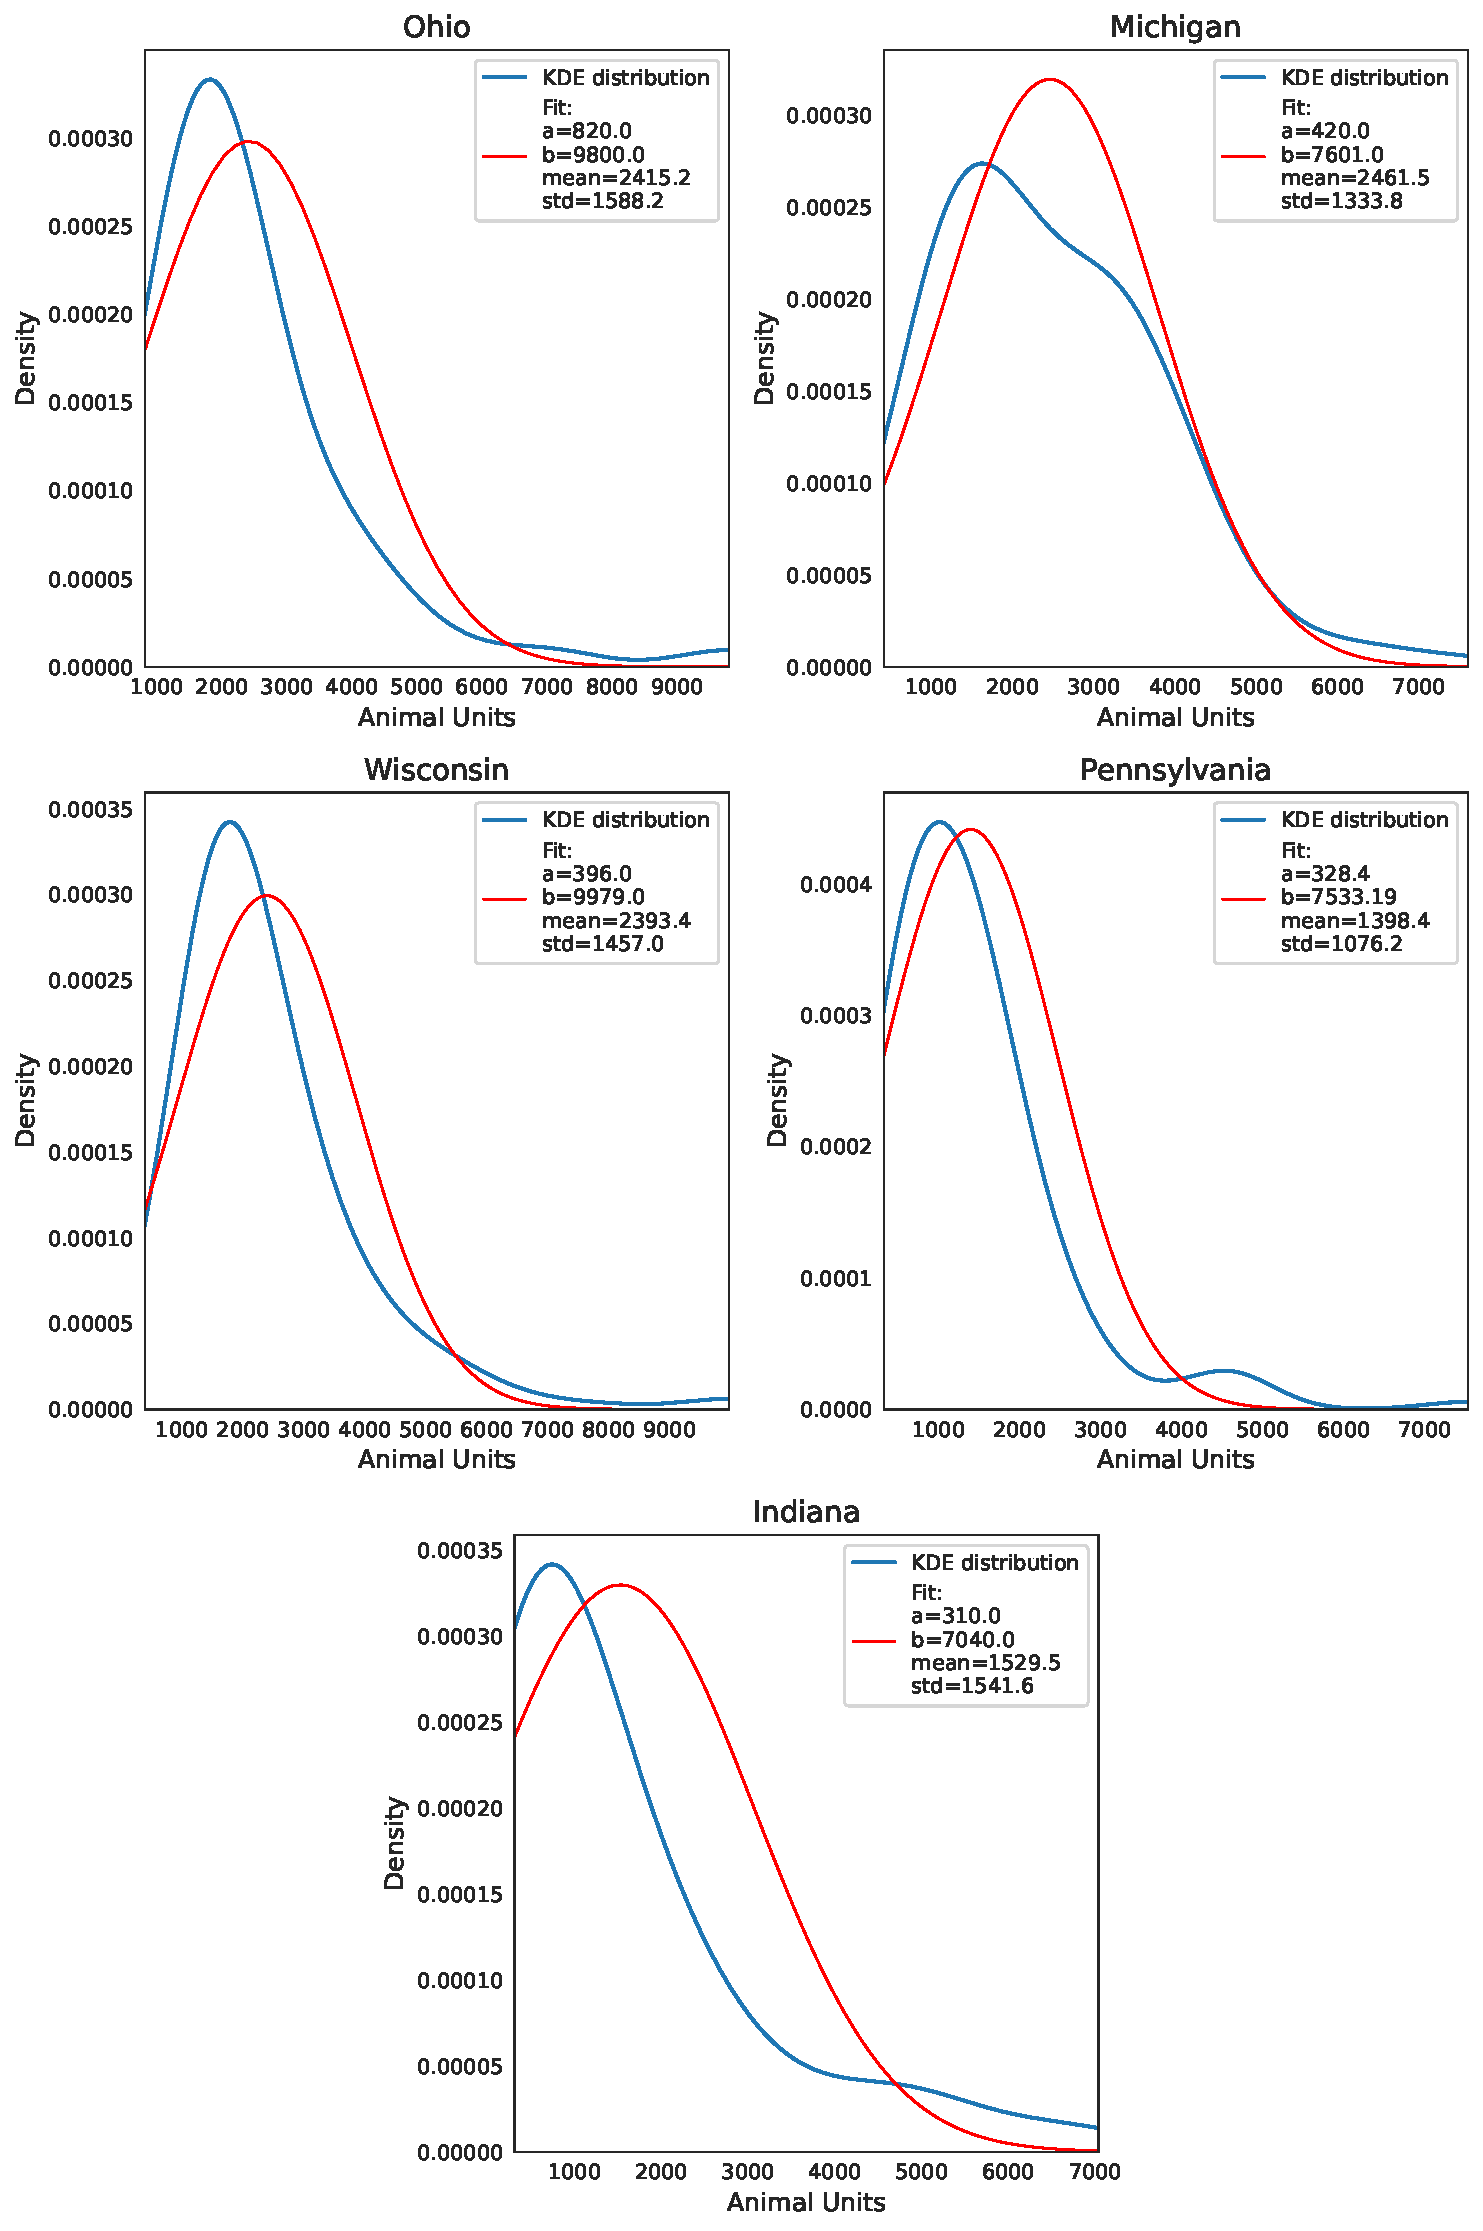
\includegraphics[width=0.81\linewidth, trim={0cm 0cm 0cm 0cm},clip]{SupMat_Figures/CAFOs_Size_Distribution} 
%	\caption{Distribution of CAFOs size in regions of the the Great Lakes area.}
%	\label{fig:CAFOsSizeDist}
%\end{figure}

\newpage
\section{Slaughter industry}
Table \ref{table:SlaughterAnimals} collects the number of animals slaughtered and the phosphorus in slaughterhouse waste in the province of Ontario for year 2019.

\begin{table}[h]
	\centering
	\caption{Truncated normal distribution fitting parameters for the distribution of cAFOs sizes in regions of the Great Lakes area.} \label{table:SlaughterAnimals}
	\resizebox{0.99\columnwidth}{!}{
		%		\begin{threeparttable}
		\begin{tabular}{@{}lcccccc@{}}
			\toprule
			& Cattle  & Swine     & Sheep   & Rabbit        & Poultry                                                                         & Total                        \\ \midrule
			\begin{tabular}[c]{@{}l@{}}Animals slaughtered in federally\\ licensed facilities (heads, 2019)\end{tabular}    & 628,366 & 4,010,926 & 84,721  & Not available & \multirow{2}{*}{\begin{tabular}[c]{@{}c@{}}238,979,246 \\ (total)\end{tabular}} & \multirow{2}{*}{244,663,410} \\
			\begin{tabular}[c]{@{}l@{}}Animals slaughtered in provincially\\ licensed facilities (heads, 2019)\end{tabular} & 99,561  & 368,267   & 266,946 & 225,377       &                                                                                 &                              \\
			\begin{tabular}[c]{@{}l@{}}P flows through slaughterhouse\\ waste in t (2019)\end{tabular}                      & 2,222   & 621       & 42      & 7.3           & 904                                                                             & 3,796.6                      \\ \bottomrule
		\end{tabular}
		%			\begin{tablenotes}
		%				\footnotesize
		%				\item 1: \citet{MilkOntario}
		%			\end{tablenotes}
		%	\end{threeparttable}
	}
\end{table}
	
%\bibliographystyle{apacite}
%\bibliographystyle{ieee}
\bibliography{references}
	
\end{document}